Småsignalmodellen brukes til å se hvordan en transistor
reagerer på små signaler ved å dele transistoren i to deler.
En dynamisk motstand $r_\pi$ mellom base-emitter.
Og en strømgenerator mellom collector-emitter.
Strømgeneratorens strøm bestemmes av transistorens
transkonduktans $g_m$ (steilhet).
\\\\
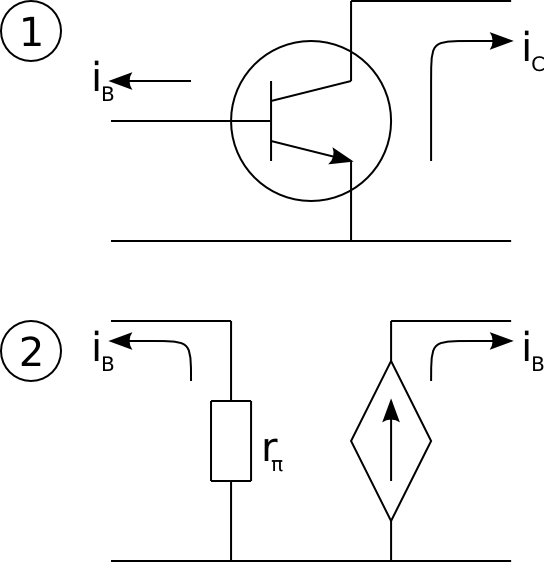
\includegraphics[width=0.5\textwidth]{./img/smasignal}
\\\\
$$i_C = \beta \cdot i_B$$
$$i_C = g_m \cdot V_{BE}$$



\subsubsection{Transkonduktans - Steilhet}
Steilhet $g_m$, eller bratthet, er hvor bratt strømmen stiger.
Med andre ord tangenten.
$g_m$ benevnes i Siemens.
$$g_m = \frac{\Delta I_C}{\Delta V_{BE}}$$
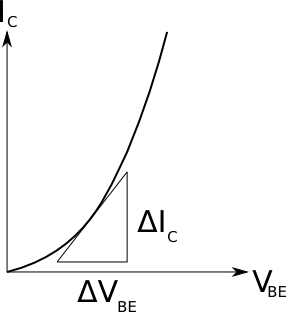
\includegraphics[width=0.5\textwidth]{./img/steilhet}
\\\\
Strømmen $I_C$ er gitt ved
$$I_C = \alpha \cdot I_{ES} \cdot e^{\sfrac{V_{BE}}{V_T}}$$
\\
Vi finner $g_m$ ved å derivere $I_C$.
$$g_m = \frac{\Delta I_C}{\Delta V_{BE}}
= \alpha \cdot I_{ES} \cdot e^{\sfrac{V_{BE}}{V_T}} \cdot \frac{1}{V_T}
= I_C \cdot \frac{1}{V_T} = \frac{I_C}{V_T}$$
Hvor $V_T = 25mV$.



\subsubsection{Dynamisk inngangsresistans}
TODO
